% ==================== NOI DUNG CHINH ====================
\section{Giới thiệu}

Trong dòng chảy của lịch sử kiến trúc và xây dựng, các công trình có cấu trúc bề mặt cong phức tạp luôn là một thách thức lớn đối với các kỹ sư và nhà thiết kế. Từ các đường hầm xuyên qua lòng núi tuyết hiểm trở, các vòm cầu đá cổ kính nâng đỡ những tuyến đường huyết mạch, cho đến các cấu trúc cầu thang xoắn ốc hiện đại đầy tính nghệ thuật trong các tòa nhà thông minh – tất cả đều sở hữu những hình dáng hình học không tiêu chuẩn. Việc xác định chính xác các thông số vật lý của chúng, đặc biệt là diện tích bề mặt, đóng vai trò sống còn trong việc tính toán tải trọng, dự toán định mức vật liệu thi công, cũng như lập kế hoạch tối ưu hóa chi phí sản xuất.

Tuy nhiên, các phương pháp hình học sơ cấp hoàn toàn bất lực trước các bề mặt cong thay đổi liên tục trong không gian ba chiều. Để giải quyết triệt để bài toán này, việc ứng dụng các công cụ toán học cao cấp là điều tất yếu. Trong đó, phép tính tích phân mặt – bao gồm tích phân mặt loại một và phương pháp tham số hóa bề mặt – chính là chìa khóa lý thuyết mạnh mẽ nhất để chuyển đổi các mô hình hình học phức tạp thành các biểu thức đại số có thể tính toán chính xác.

Nhằm làm sáng tỏ mối liên hệ mật thiết giữa toán học thuần túy và kỹ thuật thực tiễn, bài tập lớn này tập trung nghiên cứu, phân tích và giải quyết ba bài toán mô hình hóa cụ thể:
\begin{itemize}
	\item \textbf{Bài toán 1 - Mô hình đường hầm núi tuyết:} Ứng dụng trực tiếp của tích phân mặt loại một để tính toán diện tích vòm hầm chịu lực dưới các điều kiện biên hình học phức tạp.
	\item \textbf{Bài toán 2 - Mô hình cầu đá:} Sử dụng phương pháp tham số hóa bề mặt để mô tả các cấu trúc vòm cong cổ điển, từ đó xác định diện tích bề mặt tiếp xúc và bao phủ.
	\item \textbf{Bài toán 3 - Bài toán Cầu thang:} Khảo sát các cấu trúc dạng xoắn hoặc bậc thang phi tuyến tính trong kiến trúc hiện đại, một ứng dụng thực tế đòi hỏi sự kết hợp linh hoạt giữa giải tích và tư duy không gian.
\end{itemize}

Bên cạnh việc giải quyết các bài toán bằng phương pháp giải tích truyền thống nhằm tìm ra nghiệm chính xác, đề tài này còn ứng dụng công cụ lập trình phần mềm MATLAB. Việc mô phỏng trực quan hóa hình ảnh không gian 3D và tính toán số học trên MATLAB không chỉ giúp kiểm chứng tính đúng đắn của các kết quả lý thuyết, mà còn mở ra hướng tiếp cận hiện đại trong việc tự động hóa xử lý các bài toán kỹ thuật thực tế của người kỹ sư tương lai.
% =========================================================
\newpage
\section{Cơ sở lý thuyết}

% ---------------------------------------------------------
\subsection{Tích phân mặt loại 1}
\subsubsection{Định nghĩa}

% Hình 1: Sau phần Định nghĩa (tổng Riemann)
\begin{figure}[h!]
	\centering
	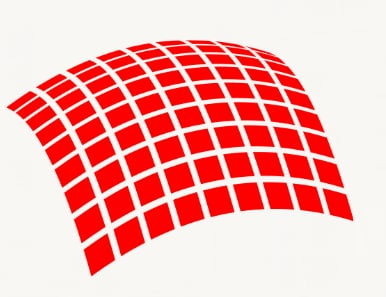
\includegraphics[width=0.55\linewidth]{figures_tech/a.jpg}
	\caption{Mô hình hóa việc chia nhỏ mặt cong \( S \) để định nghĩa tích phân mặt loại 1}
	\label{fig:chia-mat}
\end{figure}
Giả sử mặt \( S \) được biểu diễn bởi một phương trình vectơ trong không gian ba chiều:
\[
\mathbf{r}(u,v) = x(u,v)\mathbf{i} + y(u,v)\mathbf{j} + z(u,v)\mathbf{k}
\]

Đầu tiên, giả sử miền tham số \( D \) là một hình chữ nhật. Chúng ta chia miền \( D \) này thành các hình chữ nhật con \( R_{ij} \) với kích thước \( \Delta u \) theo chiều \( u \) và \( \Delta v \) theo chiều \( v \). Tương ứng với phép chia trên mặt phẳng này, mặt không gian \( S \) cũng bị chia thành các mảnh cong nhỏ tương ứng, ký hiệu là \( S_{ij} \). \\

Với một hàm số ba biến \( f(x,y,z) \) có tập xác định chứa mặt \( S \), ta chọn một điểm đại diện bất kỳ \( (x_{ij}^{*}, y_{ij}^{*}, z_{ij}^{*}) \in S_{ij} \). Sau đó, ta đánh giá giá trị của hàm tại điểm này, nhân với diện tích \( \Delta S_{ij} \) của chính mảnh đó, và thiết lập tổng Riemann:
\[
\sum_{i=1}^{m} \sum_{j=1}^{n} f(x_{ij}^{*}, y_{ij}^{*}, z_{ij}^{*}) \Delta S_{ij}
\]

Bằng cách chuyển qua giới hạn khi số lượng các mảnh mặt cong tăng lên vô hạn (nghĩa là kích thước các mảnh tiến về 0), ta định nghĩa tích phân mặt của hàm \( f \) trên mặt \( S \) là:
\[
\iint_{S} f(x,y,z) \, dS = \lim_{m,n \to \infty} \sum_{i=1}^{m} \sum_{j=1}^{n} f(x_{ij}^{*}, y_{ij}^{*}, z_{ij}^{*}) \Delta S_{ij}
\]

\subsubsection{Cách tính}
Để tính tích phân mặt loại một, ta cần chiếu mặt cong \( S \) xuống một trong các mặt phẳng tọa độ để đưa về tích phân kép. Có 3 trường hợp:

\begin{itemize}
	\item \textbf{Trường hợp 1:} Mặt cong \( S \) cho bởi phương trình \( z = z(x,y) \), gọi \( D_{xy} \) là hình chiếu của \( S \) xuống mặt phẳng \( Oxy \). Khi đó:
	\[
	dS = \sqrt{1 + \left( \frac{\partial z}{\partial x} \right)^2 + \left( \frac{\partial z}{\partial y} \right)^2} \, dx\,dy
	\]
	\[
	\iint_{S} f(x,y,z) \, dS = \iint_{D_{xy}} f\bigl(x, y, z(x,y)\bigr) \sqrt{1 + \left( \frac{\partial z}{\partial x} \right)^2 + \left( \frac{\partial z}{\partial y} \right)^2} \, dx\,dy
	\]
	% Hình 2: Sau Trường hợp 1 (z = z(x,y))
	\begin{figure}[h!]
		\centering
		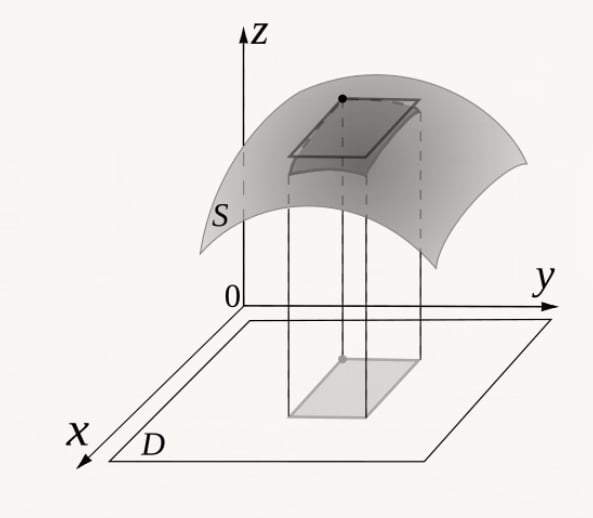
\includegraphics[width=0.55\linewidth]{figures_tech/b.jpg}
		\caption{Mối liên hệ giữa vi phân diện tích trên mặt cong \( dS \) và vi phân diện tích trên hình chiếu \( dx\,dy \)}
		\label{fig:ds-dxdy}
	\end{figure}
	\item \textbf{Trường hợp 2:} Mặt cong \( S \) cho bởi phương trình \( y = y(x,z) \), gọi \( D_{xz} \) là hình chiếu của \( S \) xuống mặt phẳng \( Oxz \). Khi đó:
	\[
	dS = \sqrt{1 + \left( \frac{\partial y}{\partial x} \right)^2 + \left( \frac{\partial y}{\partial z} \right)^2} \, dx\,dz
	\]
	\[
	\iint_{S} f(x,y,z) \, dS = \iint_{D_{xz}} f\bigl(x, y(x,z), z\bigr) \sqrt{1 + \left( \frac{\partial y}{\partial x} \right)^2 + \left( \frac{\partial y}{\partial z} \right)^2} \, dx\,dz
	\] \\
	
	\item \textbf{Trường hợp 3:} Mặt cong \( S \) cho bởi phương trình \( x = x(y,z) \), gọi \( D_{yz} \) là hình chiếu của \( S \) xuống mặt phẳng \( Oyz \). Khi đó:
	\[
	dS = \sqrt{1 + \left( \frac{\partial x}{\partial y} \right)^2 + \left( \frac{\partial x}{\partial z} \right)^2} \, dy\,dz
	\]
	\[
	\iint_{S} f(x,y,z) \, dS = \iint_{D_{yz}} f\bigl(x(y,z), y, z\bigr) \sqrt{1 + \left( \frac{\partial x}{\partial y} \right)^2 + \left( \frac{\partial x}{\partial z} \right)^2} \, dy\,dz
	\]
\end{itemize}

\subsubsection{Phân biệt tích phân mặt loại I và loại II}
Dựa vào giáo trình, ta có thể rút ra các điểm khác biệt cơ bản sau giữa tích phân mặt loại I và loại II:

\begin{itemize}
	\item \textbf{Về bản chất đại lượng:} Tích phân mặt loại I đặc trưng cho các đại lượng \emph{vô hướng} (như tính diện tích mặt cong, hoặc khối lượng của mặt cong khi biết hàm mật độ \( f(x,y,z) \)). Trong khi đó, tích phân mặt loại II dùng để giải quyết bài toán của đại lượng có hướng như tính lượng chất lỏng (thông lượng) đi qua một bề mặt cho trước.
	
	\item \textbf{Sự phụ thuộc vào hướng của mặt:} Tích phân mặt loại I tính trên mặt cong \( S \) thông thường (không cần định hướng). Ngược lại, tích phân mặt loại II phụ thuộc chặt chẽ vào mặt định hướng (mặt trơn hai phía, được xác định bởi pháp vectơ đơn vị \( \mathbf{n} \)). Nếu đổi hướng của pháp vectơ (chọn phía mặt cong ngược lại), giá trị của tích phân mặt loại II sẽ đổi dấu.
\end{itemize} 
\newpage
\subsubsection{Ví dụ minh họa}

\textbf{Ví dụ:}
Tính $I = \iint_{S} xyz\; dS$, trong đó $S$ là phần mặt phẳng $x+y+z=1$
nằm trong góc $x \ge 0,\; y \ge 0,\; z \ge 0$.% [cite: 198, 199, 200]

\medskip
\textbf{Giải:}
Mặt cong $S$ được xác định bởi phương trình $z = 1-x-y$.% [cite: 203]
Ta tính các đạo hàm riêng:
\[
z'_x = -1, \qquad z'_y = -1.
% [cite: 203, 204]
\]
Hình chiếu của mặt $S$ xuống mặt phẳng $Oxy$ là miền $D$ giới hạn bởi
$x \ge 0,\; y \ge 0$ và đường thẳng $x+y=1$.% [cite: 205]
Áp dụng công thức tích phân mặt loại một:% [cite: 206]

\begin{equation}
	I \;=\;
	\iint_{D}
	xy\,(1-x-y)
	\sqrt{1 + (z'_x)^2 + (z'_y)^2}\; dx\,dy
	% [cite: 207]
\end{equation}

\begin{equation}
	I \;=\;
	\iint_{D}
	xy\,(1-x-y)
	\sqrt{1 + (-1)^2 + (-1)^2}\; dx\,dy
	\;=\;
	\sqrt{3}
	\iint_{D}
	\left(xy - x^2 y - x y^2\right) dx\,dy
	% [cite: 208]
\end{equation}

Chuyển về tích phân lặp trên miền $D$:% [cite: 209]

\begin{align*}
	I
	&= \sqrt{3}
	\int_{0}^{1} dx
	\int_{0}^{1-x}
	\left(xy - x^2 y - x y^2\right) dy
	\\[6pt] % [cite: 210]
	&= \sqrt{3}
	\int_{0}^{1}
	\left[
	x\,\frac{y^2}{2} - x^2\,\frac{y^2}{2} - x\,\frac{y^3}{3}
	\right]_{y=0}^{y=1-x} dx
	\\[6pt] % [cite: 211]
	&= \sqrt{3}
	\int_{0}^{1}
	\left[
	\frac{x(1-x)^2}{2}
	- \frac{x^2(1-x)^2}{2}
	- \frac{x(1-x)^3}{3}
	\right] dx
	\;=\;
	\frac{\sqrt{3}}{120}
	% [cite: 211, 212]
\end{align*}

% ---------------------------------------------------------
\newpage
\subsection{Tham số hoá bề mặt}

\subsubsection{Giới thiệu qua tham số hoá}

\begin{figure}[H]
	\centering
	
\includegraphics[width=0.7\linewidth]{figures_tech/1.jpg} 
	\caption{Quỹ đạo chất điểm là đường cong C không thể được biểu diễn bởi 1 hàm số} % Thay bằng mô tả thực tế
	\label{fig:sample_image} % Nhãn để tham chiếu
\end{figure}


Một hàm số $y=f(x)$ có thể biểu diễn một đường cong trong không gian hai chiều $Oxy$.% [cite: 67]
Thế nhưng không phải đường cong nào cũng có thể được biểu diễn bởi một hàm số.% [cite: 68]
Ví dụ như một chất điểm chuyển động trong không gian hai chiều có đường cong $C$
không thể biểu diễn bằng hàm số dạng $y=f(x)$
(tồn tại nơi mà cùng hoành độ $x$ có nhiều giá trị $y$ tương ứng).% [cite: 69]
Thế nhưng, ta biết vận tốc của chất điểm đang chuyển động có thể tách thành hai thành phần
$v_x(t)$ và $v_y(t)$ là các hàm số theo thời gian.% [cite: 70]
Theo đó, ta cũng biểu diễn được tọa độ $x$ và $y$ của chất điểm là các hàm số theo thời gian
và từ đó biểu diễn được đường cong $C$ bằng các hàm số theo một biến số mới là thời gian.% [cite: 71]

Từ ý tưởng đó, ta có thể biểu diễn một đường cong trong mặt phẳng tọa độ bằng cách biểu diễn
tọa độ của một điểm trên đường cong bằng các hàm số theo một biến số mới.% [cite: 72]
Đặt $x,\,y$ là các hàm số theo biến số mới $t$:% [cite: 73]

\begin{equation}
	x = f(t), \qquad y = g(t)
	% [cite: 74]
\end{equation}

Khi giá trị $t$ thay đổi, tọa độ điểm $(x,y)$ sẽ di chuyển và vạch ra đường cong $C$.% [cite: 76]
Ta gọi $t$ là \emph{tham số}, đường cong $C$ là \emph{đường cong tham số}
và phương trình trên là \emph{phương trình tham số}.% [cite: 76]
Tương tự, ta có thể biểu diễn một đường cong trong không gian bằng phương trình tham số
cho ba biến tọa độ $x,\,y,\,z$ phụ thuộc một tham số $t$.% [cite: 77]
Ta gọi quá trình trên là \emph{tham số hóa đường cong}.% [cite: 78]
\newpage
\subsubsection{Tham số hoá mặt phẳng}

Ở trên ta đã đề cập cách tham số hoá một đường cong trong không gian;
ta cũng có thể tham số hoá một mặt cong bằng phương trình tham số
với hai tham số khác nhau.% [cite: 81, 82]
Đặt vector vị trí một điểm trên mặt phẳng là $\mathbf{r}$:% [cite: 83]

\begin{equation}
	\mathbf{r}(u,v)
	\;=\; x(u,v)\,\mathbf{i}
	+ y(u,v)\,\mathbf{j}
	+ z(u,v)\,\mathbf{k}
	% [cite: 84]
\end{equation}

Từ đó ta cũng có phương trình tham số cho mặt cong:
$x = x(u,v)$, $y = y(u,v)$, $z = z(u,v)$.% [cite: 86--89]
Vì mỗi phần tử của vector $\mathbf{r}$ là một hàm số theo hai tham số $u,v$,
nên ứng với mỗi cặp giá trị $(u,v)$ có một điểm có vector vị trí $\mathbf{r}$
khác nhau trong không gian $Oxyz$.% [cite: 90]
Nếu quét giá trị $(u,v)$ nằm trong miền $D$ của tham số $u,\,v$,
ta thu được một mặt cong $S$ trong không gian $Oxyz$.% [cite: 91]
Ta gọi mặt $S$ là \emph{bề mặt tham số}.% [cite: 91]


\begin{figure}[H]
	\centering
	
\includegraphics[width=0.7\linewidth]{figures_tech/2.jpg} 
	\caption{Miền xác định D của u,v và mặt phẳng tham số S} % Thay bằng mô tả thực tế
	\label{fig:sample_image} % Nhãn để tham chiếu
\end{figure}




Nếu ta cố định $u$ hoặc $v$ và thay đổi giá trị còn lại trong miền $D$,
ta đang vạch ra một đường cong tham số trong $Oxyz$.% [cite: 102]
Khi ta cố định $u = u_0$ và thay đổi $v$,
ta vạch ra đường cong $C_1$ trên $S$;
tương tự, cố định $v = v_0$ và thay đổi $u$ cho đường cong $C_2$.% [cite: 103]
Ta có thể xem việc tham số hoá mặt $S$ như là việc phác hoạ mặt $S$
bằng cách kẻ nhiều đường cong tham số $C_1$ với các giá trị $u$ khác nhau
(hay nhiều $C_2$ với các giá trị $v$ khác nhau).% [cite: 104]
\begin{figure}[H]
	\centering
	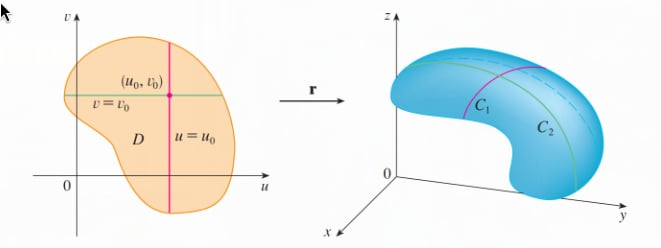
\includegraphics[width=0.7\linewidth]{figures_tech/3.jpg} 
	\caption{Quỹ đạo chất điểm là đường cong C không thể được biểu diễn bởi 1 hàm số} % Thay bằng mô tả thực tế
	\label{fig:sample_image} % Nhãn để tham chiếu
\end{figure}


Đường cong $C_1$ và $C_2$ ở trên được gọi là \emph{đường cong trên lưới} (grid curves).% [cite: 121]
Thực tế khi dùng máy tính dựng các bề mặt tham số thì các đường cong trên
sẽ được vẽ trên bề mặt để dễ nhìn, hình dung và khảo sát hơn.% [cite: 122]
\begin{figure}[H]
	\centering
	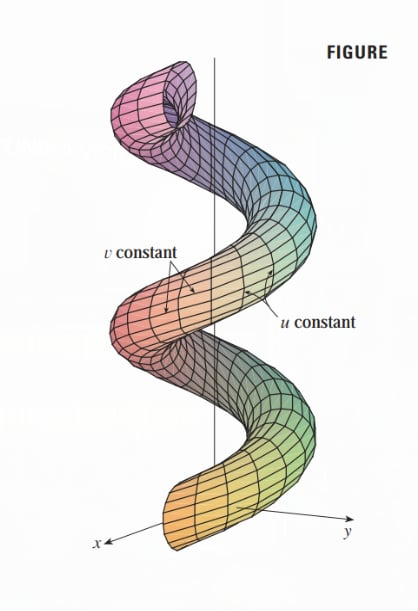
\includegraphics[width=0.3\linewidth]{figures_tech/4.jpg} 
	\caption{Biểu diễn lưới tọa độ trên bề mặt để mô tả cấu trúc của một mặt cong 3D phức tạp} % Thay bằng mô tả thực tế
	\label{fig:sample_image} % Nhãn để tham chiếu
\end{figure}

\subsubsection{Tính diện tích bề mặt tham số hoá}
\begin{figure}[H]
	\centering
	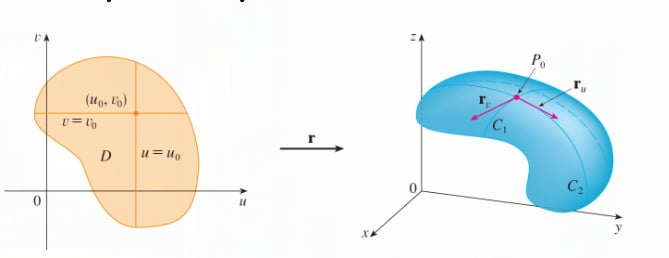
\includegraphics[width=0.7\linewidth]{figures_tech/5.jpg} 
	\caption{Biểu diễn vector tiếp tuyến của các đường cong trên lưới từ điểm đang xét} % Thay bằng mô tả thực tế
	\label{fig:sample_image} % Nhãn để tham chiếu
\end{figure}

Vị trí điểm $P_0$ bất kì nằm trên mặt $S$ được biểu diễn bằng
vector vị trí $\mathbf{r} = \overrightarrow{OP_0}$
tương ứng với $u = u_0$, $v = v_0$.% [cite: 137]
Khi ta cố định $u = u_0$ thì vector vị trí $\mathbf{r}(u_0, v)$
là một hàm vector với một tham số $v$ và vạch ra đường cong $C_1$.% [cite: 138]
Từ đó ta xác định được vector tiếp tuyến đường cong $C_1$ tại $P_0$
bằng cách lấy đạo hàm riêng của $\mathbf{r}$ theo $v$:% [cite: 138]

\begin{equation}
	\mathbf{r}_v
	\;=\; \frac{\partial x}{\partial v}(u_0,v_0)\,\mathbf{i}
	+ \frac{\partial y}{\partial v}(u_0,v_0)\,\mathbf{j}
	+ \frac{\partial z}{\partial v}(u_0,v_0)\,\mathbf{k}
	% [cite: 140]
\end{equation}

Tương tự, khi ta cố định $v = v_0$ ta có vector tiếp tuyến với $C_2$ tại $P_0$:% [cite: 141]

\begin{equation}
	\mathbf{r}_u
	\;=\; \frac{\partial x}{\partial u}(u_0,v_0)\,\mathbf{i}
	+ \frac{\partial y}{\partial u}(u_0,v_0)\,\mathbf{j}
	+ \frac{\partial z}{\partial u}(u_0,v_0)\,\mathbf{k}
	% [cite: 141]
\end{equation}

Nếu tích hữu hướng $\mathbf{r}_u \times \mathbf{r}_v \ne \mathbf{0}$
thì ta gọi mặt cong đó là \emph{mặt cong trơn}.% [cite: 142]
Với mặt cong trơn thì mặt phẳng tiếp tuyến tại $P_0$
phải chứa hai vector $\mathbf{r}_u$ và $\mathbf{r}_v$.% [cite: 143]

\begin{figure}[H]
	\centering
	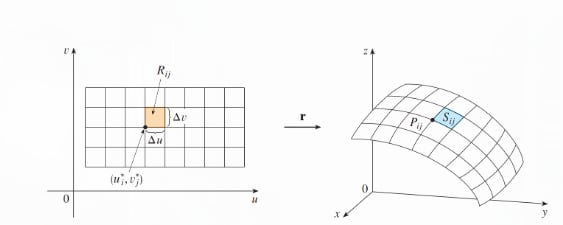
\includegraphics[width=0.7\linewidth]{figures_tech/6.jpg} 
	\caption{Phân hoạch miền D và mảng diện tích nhỏ tương ứng trên mặt S} % Thay bằng mô tả thực tế
	\label{fig:sample_image} % Nhãn để tham chiếu
\end{figure}



Khi ta phân hoạch miền $D$ thành các ô hình chữ nhật nhỏ với các cạnh $\Delta u$ và $\Delta v$,
thì bề mặt $S$ cũng bị phân hoạch thành các ``ô lưới''.% [cite: 151]
Xét một ô lưới có diện tích nhỏ $S_{ij}$ trên mặt $S$ được xét từ điểm $P_{ij}$
(tương ứng với $u = u_i^{*}$, $v = v_j^{*}$),
ta có thể xấp xỉ mảng diện tích nhỏ này bằng một tích hữu hướng:% [cite: 152]

\begin{equation}
	\bigl|(\Delta u\,\mathbf{r}_u^{*}) \times (\Delta v\,\mathbf{r}_v^{*})\bigr|
	\;=\;
	\bigl|\mathbf{r}_u^{*} \times \mathbf{r}_v^{*}\bigr|\,\Delta u\,\Delta v
	% [cite: 153]
\end{equation}

Có thể thấy $\mathbf{r}_u^{*} \times \mathbf{r}_v^{*}$
chính là vector pháp tuyến $\mathbf{n}$ của mặt $S$ tại $P_{ij}$.\\% [cite: 154]

\begin{figure}[H]
	\centering
	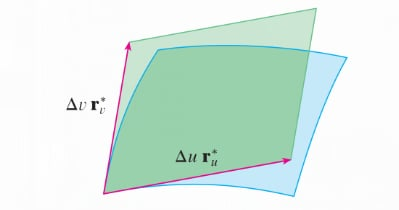
\includegraphics[width=0.7\linewidth]{figures_tech/7.jpg} 
	\caption{Xấp xỉ mảng diện tích nhỏ Sij bằng một tích hữu hướng} % Thay bằng mô tả thực tế
	\label{fig:sample_image} % Nhãn để tham chiếu
\end{figure}

Ta có thể xấp xỉ như trên vì khi $\Delta u$ và $\Delta v$ đủ nhỏ,
diện tích mảng $S_{ij}$ rất nhỏ và độ ``vênh'' của nó không đáng kể.% [cite: 157]
Theo đó, diện tích mặt $S$ được xấp xỉ bằng:% [cite: 158]

\begin{equation}
	\sum_{i=1}^{m} \sum_{j=1}^{n}
	\bigl|\mathbf{r}_u^{*} \times \mathbf{r}_v^{*}\bigr|\,\Delta u\,\Delta v
	% [cite: 159]
\end{equation}

Khi $\Delta u$ và $\Delta v$ ngày càng nhỏ,
công thức tính diện tích trở thành:% [cite: 160]

\begin{equation}
	A(S) \;=\; \iint_{D} \bigl|\mathbf{r}_u \times \mathbf{r}_v\bigr|\; dA
	% [cite: 162]
\end{equation}

với $(u,v) \in D$ và các đạo hàm riêng tương ứng.% [cite: 161, 163]
% =========================================================
\newpage
% =========================================================
\newpage
\section{Ứng dụng thực tế}

% ---------------------------------------------------------
\subsection{BÀI TOÁN 1: Mô hình đường hầm núi tuyết (Giải bằng Tích phân mặt loại 1)}

\textbf{Đề bài:}
Mô hình đường hầm núi tuyết ở Vân Nam (Trung Quốc) có thiết kế như hình bên dưới.
Giả sử, ta có mô hình đường hầm với $S$ là phần mặt trụ $x^2 + z^2 = 1$
bị chắn bởi các mặt phẳng $y + z = 2$, $y = 0$ và $z \ge 0$ (đơn vị đo trên các trục tọa độ là mét).
Để chống vỡ nứt do nhiệt độ thấp, nhà thầu cần thi công phủ một lớp vật liệu cách nhiệt lên toàn bộ bề mặt $S$ của đường hầm.
Do đặc thù địa hình, càng đi sâu vào trong hầm (theo chiều dương của trục $y$) việc vận chuyển vật liệu và thi công càng khó khăn, dẫn đến đơn giá thi công tăng dần.
Giả sử chi phí để hoàn thiện $1m^2$ bề mặt tại điểm $M(x, y, z)$ được tính theo hàm số:
\[
C(x, y, z) = 100 + 50y \quad (\text{triệu VNĐ}/m^2)
\]
Dùng tích phân mặt, hãy tính tổng chi phí dự kiến để thi công lớp phủ cách nhiệt cho toàn bộ bề mặt đường hầm trên.

\begin{figure}[H]
	\centering
	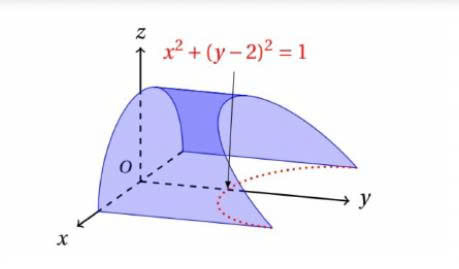
\includegraphics[width=0.7\linewidth]{figures_tech/a1.jpg} 
	\caption{Bài toán 1}
	\label{fig:tunnel_real}
\end{figure}
\newpage
\subsubsection{Lời giải chi tiết bằng giải tích}

Mặt cong $S$ là phần mặt trụ $x^2 + z^2 = 1$ ở phía trên mặt phẳng $Oxy$ ($z \ge 0$),
suy ra phương trình mặt $S$ là $z = \sqrt{1-x^2}$.

Hình chiếu $D_{xy}$ của mặt $S$ xuống mặt phẳng $Oxy$ bị giới hạn bởi:
\[
y = 0, \qquad
y = 2 - z = 2 - \sqrt{1-x^2}, \qquad
x \in [-1,\,1].
\]

Vi phân diện tích $dS$ tính theo mặt $z(x,y)$:
\begin{equation}
	dS
	\;=\; \sqrt{1 + (z'_x)^2 + (z'_y)^2}\; dx\,dy
	\;=\; \sqrt{1 + \left(\frac{-x}{\sqrt{1-x^2}}\right)^{\!2} + 0}\; dx\,dy
	\;=\; \frac{1}{\sqrt{1-x^2}}\; dx\,dy
\end{equation}

Áp dụng công thức tích phân mặt loại 1, tổng chi phí thi công lớp cách nhiệt mặt hầm:
\begin{equation}
	T
	\;=\; \iint_{D_{xy}} (100 + 50y) \frac{1}{\sqrt{1-x^2}}\; dx\,dy
	\;=\; \int_{-1}^{1} \left( \int_{0}^{\,2-\sqrt{1-x^2}} \frac{100 + 50y}{\sqrt{1-x^2}}\; dy \right) dx
\end{equation}

Tính tích phân lớp trong theo biến $y$:
\begin{equation}
	\int_{0}^{\,2-\sqrt{1-x^2}} (100 + 50y)\; dy 
	\;=\; \Bigl[100y + 25y^2\Bigr]_{0}^{\,2-\sqrt{1-x^2}}
\end{equation}
\[
\;=\; 100\left(2 - \sqrt{1-x^2}\right) + 25\left(2 - \sqrt{1-x^2}\right)^2
\;=\; 325 - 200\sqrt{1-x^2} - 25x^2
\]

Thay kết quả vừa tính vào phương trình tổng chi phí, ta thu được tích phân theo biến $x$:
\begin{equation}
	T
	\;=\; \int_{-1}^{1} \frac{325 - 200\sqrt{1-x^2} - 25x^2}{\sqrt{1-x^2}}\; dx
	\;=\; \int_{-1}^{1} \frac{325 - 25x^2}{\sqrt{1-x^2}}\; dx - \int_{-1}^{1} 200\; dx
\end{equation}

Tính riêng từng thành phần tích phân, ta có:
\[
\int_{-1}^{1} 200\; dx \;=\; 400
\]

Đối với số hạng tích phân thứ nhất, ta thực hiện đổi biến lượng giác bằng cách đặt $x = \sin t \Rightarrow dx = \cos t\,dt$. 
Đổi cận: với $x = -1 \Rightarrow t = -\frac{\pi}{2}$; với $x = 1 \Rightarrow t = \frac{\pi}{2}$. Khi đó phương trình trở thành:
\begin{equation}
	\int_{-1}^{1} \frac{325 - 25x^2}{\sqrt{1-x^2}}\; dx
	\;=\; \int_{-\pi/2}^{\pi/2} \frac{325 - 25\sin^2 t}{\cos t} \cos t\,dt
	\;=\; \int_{-\pi/2}^{\pi/2} (325 - 25\sin^2 t)\,dt
\end{equation}
\begin{equation}
	\;=\; \int_{-\pi/2}^{\pi/2} \left( \frac{625}{2} + \frac{25}{2}\cos 2t \right) dt
	\;=\; \left[ \frac{625}{2}t + \frac{25}{4}\sin 2t \right]_{-\pi/2}^{\pi/2}
	\;=\; \frac{625\pi}{2}
\end{equation}

Tổng hợp lại hai thành phần trên, ta thu được tổng chi phí dự kiến để hoàn thiện mặt hầm:
\[
T
\;=\; \frac{625\pi}{2} - 400
\;\approx\; \boxed{581.75} \quad (\text{triệu VNĐ})
\]

\subsubsection{Kết quả mô phỏng Matlab}
Để kiểm chứng lại kết quả giải tay, nhóm đã sử dụng phần mềm MATLAB để tính toán tích phân và dựng mô hình 3D cho bề mặt đường hầm. Kết quả số trị từ MATLAB cho ra tổng chi phí hoàn toàn trùng khớp với giá trị tính toán lý thuyết là $\frac{625\pi}{2} - 400 \approx 581.75$ triệu VNĐ.

\textit{(Chi tiết mã nguồn MATLAB được trình bày tại Phụ lục A.1)}

\begin{figure}[H]
	\centering
	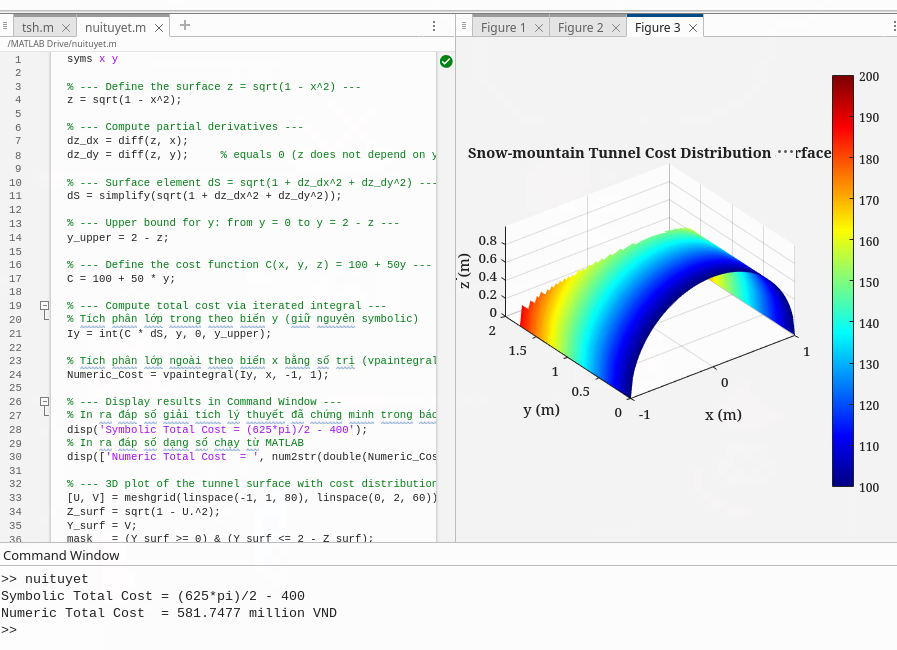
\includegraphics[width=1.0\linewidth]{figures_tech/1213.png} 
	\caption{Mô phỏng Matlab bài toán 1}
	\label{fig:matlab_tunnel}
\end{figure}
% ---------------------------------------------------------
\newpage
% ---------------------------------------------------------
\subsection{BÀI TOÁN 2: Mô hình cầu đá (Giải bằng Tham số hóa bề mặt)}

\textbf{Đề bài:}
Kiến trúc cầu đá đặc biệt phổ biến ở nhiều quốc gia trên thế giới từ thời cổ đại đến thời trung cổ là một phần quan trọng trong lịch sử xây dựng và kiến trúc. Cầu đá thường có dạng hình vòm. Giả sử một mô hình cầu đá có bề mặt cong $S$ là một phần của mặt trụ $x^2 + z^2 = 1$ bị giới hạn bởi các mặt phẳng $y = 1$, $y = 2$ và nằm phía trên mặt phẳng đất $z \ge 0$ (đơn vị đo trên các trục tọa độ là mét).
Để bảo vệ cấu trúc kiến trúc khỏi các tác động thời tiết và rêu mốc, đơn vị thi công cần phủ một lớp dung dịch hóa chất chuyên dụng lên toàn bộ bề mặt $S$ này. Do đặc thù hình học và điều kiện thi công, đơn giá hoàn thiện trên mỗi mét vuông bề mặt tại điểm $M(x, y, z)$ thay đổi liên tục theo quy luật sau:
\[
C(x, y, z) = 61 + 73y + 12z \quad (\text{triệu VNĐ}/m^2)
\]
Yêu cầu: Bằng phương pháp tham số hóa bề mặt, hãy lập mô hình toán học và tính tổng chi phí dự kiến để hoàn thành hạng mục thi công lớp phủ bảo vệ cho toàn bộ bề mặt $S$ của mô hình cầu đá.

\begin{figure}[H]
	\centering
	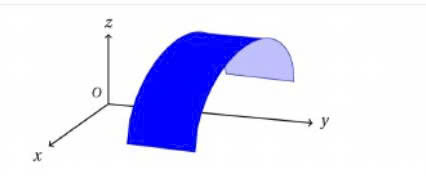
\includegraphics[width=0.7\linewidth]{figures_tech/a2.jpg} 
	\caption{Bài toán 2}
	\label{fig:bridge_real}
\end{figure}
\newpage 
\subsubsection{Lời giải chi tiết bằng giải tích}

\textbf{Xác định mặt cong $S$ và giới hạn không gian:}
Bề mặt cầu đá $S$ là một phần của mặt trụ tròn xoay có trục đối xứng trùng với trục $y$. Phương trình tổng quát: $x^2 + z^2 = R^2$ với $R = 1$.
Mặt cong bị chặn bởi hai mặt phẳng song song với mặt phẳng $(xOz)$ là $y = 1$ và $y = 2$, đồng thời nằm phía trên mặt phẳng đất ($z \ge 0$).

\bigskip
\textbf{Bước 1: Thiết lập phương trình tham số}
Để tham số hóa bề mặt cong $S$, ta chuyển sang tọa độ trụ bằng hai biến số $u$ và $v$:
\begin{equation}
	x = \cos u, \qquad z = \sin u, \qquad y = v
\end{equation}
Hàm vector biểu diễn bề mặt $S$:
\[
\mathbf{r}(u,v) \;=\; \cos u\,\mathbf{i} + v\,\mathbf{j} + \sin u\,\mathbf{k}
\]
Xác định miền biến thiên $D$ của các tham số dựa trên giới hạn hình học: Do cầu nằm phía trên mặt đất $z \ge 0$ nên $\sin u \ge 0$, suy ra $u \in [0,\pi]$; theo đề bài $y \in [1, 2]$ nên $v \in [1, 2]$.
\[
D \;=\; \bigl\{\,(u,v) \in \mathbb{R}^2 \;\big|\; 0 \le u \le \pi,\; 1 \le v \le 2 \,\bigr\}
\]

\bigskip
\textbf{Bước 2: Tính toán các vector tiếp tuyến}
Lấy đạo hàm riêng của hàm vector $\mathbf{r}(u,v)$ theo từng biến số:
\begin{align}
	\mathbf{r}_u &= \frac{\partial \mathbf{r}}{\partial u} = (-\sin u,\; 0,\; \cos u) \\[4pt]
	\mathbf{r}_v &= \frac{\partial \mathbf{r}}{\partial v} = (0,\; 1,\; 0)
\end{align}

\bigskip
\textbf{Bước 3: Tính tích có hướng và vi phân diện tích $dS$}
Tích có hướng của hai vector tiếp tuyến tạo nên vector pháp tuyến của mặt cong $S$:
\begin{equation}
	\mathbf{r}_u \times \mathbf{r}_v \;=\;
	\begin{vmatrix}
		\mathbf{i} & \mathbf{j} & \mathbf{k} \\[2pt]
		-\sin u    & 0          & \cos u     \\[2pt]
		0          & 1          & 0
	\end{vmatrix}
	\;=\; (-\cos u,\; 0,\; -\sin u)
\end{equation}
Độ lớn của vector pháp tuyến (yếu tố tỷ lệ diện tích $dS$):
\begin{equation}
	\|\mathbf{r}_u \times \mathbf{r}_v\| \;=\; \sqrt{(-\cos u)^2 + 0^2 + (-\sin u)^2} \;=\; \sqrt{\cos^2 u + \sin^2 u} \;=\; 1
\end{equation}
Từ đó, vi phân diện tích mặt được xác định là: $dS = \|\mathbf{r}_u \times \mathbf{r}_v\|\,du\,dv = du\,dv$.

\bigskip
\textbf{Bước 4: Thiết lập và tính toán tích phân xác định}
Tổng chi phí $T$ được định nghĩa bằng tích phân mặt loại 1 của hàm đơn giá $C(x, y, z)$ trên bề mặt $S$:
\begin{equation}
	T \;=\; \iint_{S} C(x, y, z)\; dS \;=\; \iint_{D} (61 + 73v + 12\sin u)\; du\,dv
\end{equation}
Ta thực hiện tính toán tích phân lặp bằng cách tích phân theo biến $u$ trước và biến $v$ sau:
\begin{equation}
	T \;=\; \int_{1}^{2} \left( \int_{0}^{\pi} (61 + 73v + 12\sin u)\; du \right) dv
\end{equation}
Tính tích phân lớp trong theo biến $u$:
\begin{equation}
	\int_{0}^{\pi} (61 + 73v + 12\sin u)\; du \;=\; \Bigl[(61 + 73v)u - 12\cos u\Bigr]_{0}^{\pi}
\end{equation}
\[
\;=\; \bigl((61 + 73v)\pi - 12\cos\pi\bigr) - \bigl(0 - 12\cos 0\bigr)
\;=\; 61\pi + 73\pi v + 12 + 12
\;=\; 73\pi v + 61\pi + 24
\]
Thay kết quả vào lớp tích phân ngoài theo biến $v$:
\begin{equation}
	T \;=\; \int_{1}^{2} (73\pi v + 61\pi + 24)\; dv \;=\; \Bigl[36.5\pi v^2 + (61\pi + 24)v\Bigr]_{1}^{2}
\end{equation}
Thế các cận vào biểu thức nguyên hàm:
\[
T \;=\; \Bigl[36.5\pi(2)^2 + (61\pi + 24)(2)\Bigr] - \Bigl[36.5\pi(1)^2 + (61\pi + 24)(1)\Bigr]
\]
\[
T \;=\; (146\pi + 122\pi + 48) - (36.5\pi + 61\pi + 24)
\]
\[
T \;=\; (268\pi + 48) - (97.5\pi + 24) \;=\; \boxed{170.5\pi + 24}
\]
Tính giá trị xấp xỉ số trị cuối cùng:
\[
T \;\approx\; 170.5 \times 3.14159 + 24 \;\approx\; \boxed{559.64} \quad (\text{triệu VNĐ})
\]
\newpage
\subsubsection{Kết quả mô phỏng Matlab}
Đoạn mã MATLAB thực hiện quá trình tham số hóa bề mặt, tích hợp hàm đơn giá thi công biến đổi và tính toán tích phân số trị cho ra kết quả hoàn toàn trùng khớp với giá trị tính toán lý thuyết là $170.5\pi + 24 \approx 559.64$ triệu VNĐ.

\textit{(Chi tiết mã nguồn MATLAB được trình bày tại Phụ lục A.2)}



\begin{figure}[H]
	\centering
	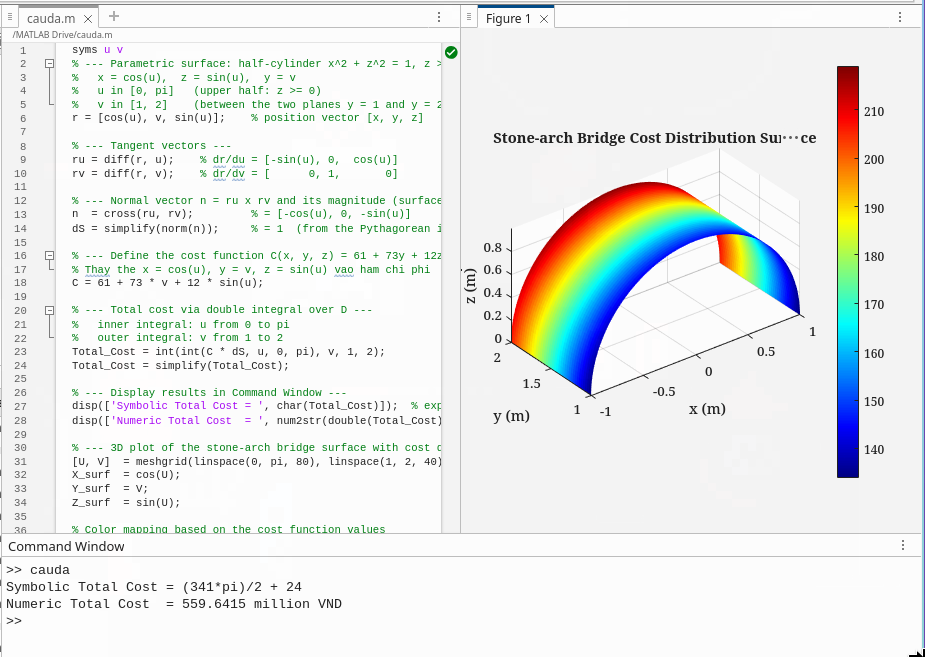
\includegraphics[width=1.0\linewidth]{figures_tech/1234.png} 
	\caption{Mô phỏng Matlab bài toán 2}
	\label{fig:matlab_bridge}
\end{figure}
\newpage
% ---------------------------------------------------------
% ---------------------------------------------------------
% ---------------------------------------------------------
\subsection{BÀI TOÁN 3: Bài toán Cầu thang}

Một ông chủ nhà giàu có muốn làm cho căn nhà sắp xây của mình một cầu thang xoắn ốc bằng bê tông. Sau khi bàn luận với đội ngũ các kỹ sư xây dựng và kiến trúc sư, họ đã chốt phương án thi công một cầu thang xoắn mà mặt cong xoắn xấp xỉ cầu thang ấy được biểu diễn trong không gian bằng phương trình tham số sau:
\[
x=u \cos(v) , \qquad y=u \sin(v) , \qquad z=h\frac{v}{2\pi}
\]
hay là
\[
\vec{r}(u,v)=\left(u \cos(v),u \sin(v),h\frac{v}{2 \pi}\right)
\]
với:
\begin{itemize}
	\item Chiều cao của thang $h=3.5$ (mét)
	\item Tham số chạy theo bề rộng thang u: $1 \le u \le 2.5$ (mét)
	\item Tham số chạy vòng xoắn của thang v: $0 \le v \le 2\pi$ (rad)
\end{itemize}

Hơn nữa, chủ nhà cũng có 1 ý muốn thẩm mỹ là bề dày lớp bê tông tính từ rìa trong ra rìa ngoài giảm dần 1 cách tuyến tính từ 35 cm đến 25 cm (bề dày tính từ mặt dưới thang đến bậc bước đi). Sau khi được các kỹ sư đưa ra các đề xuất và xác nhận tính an toàn, chủ nhà đã đồng ý dùng loại bê tông cốt thép có khối lượng riêng khoảng (theo TCVN 2737:2023 và xấp xỉ gia tốc trọng trường $g=10 m/s$) $D=2500 \frac{kg}{m^3}$. Hãy ước tính khối lượng bê tông cốt thép cần dùng để xây thang xoắn trên cho chủ nhà.

\begin{figure}[H]
	\centering
	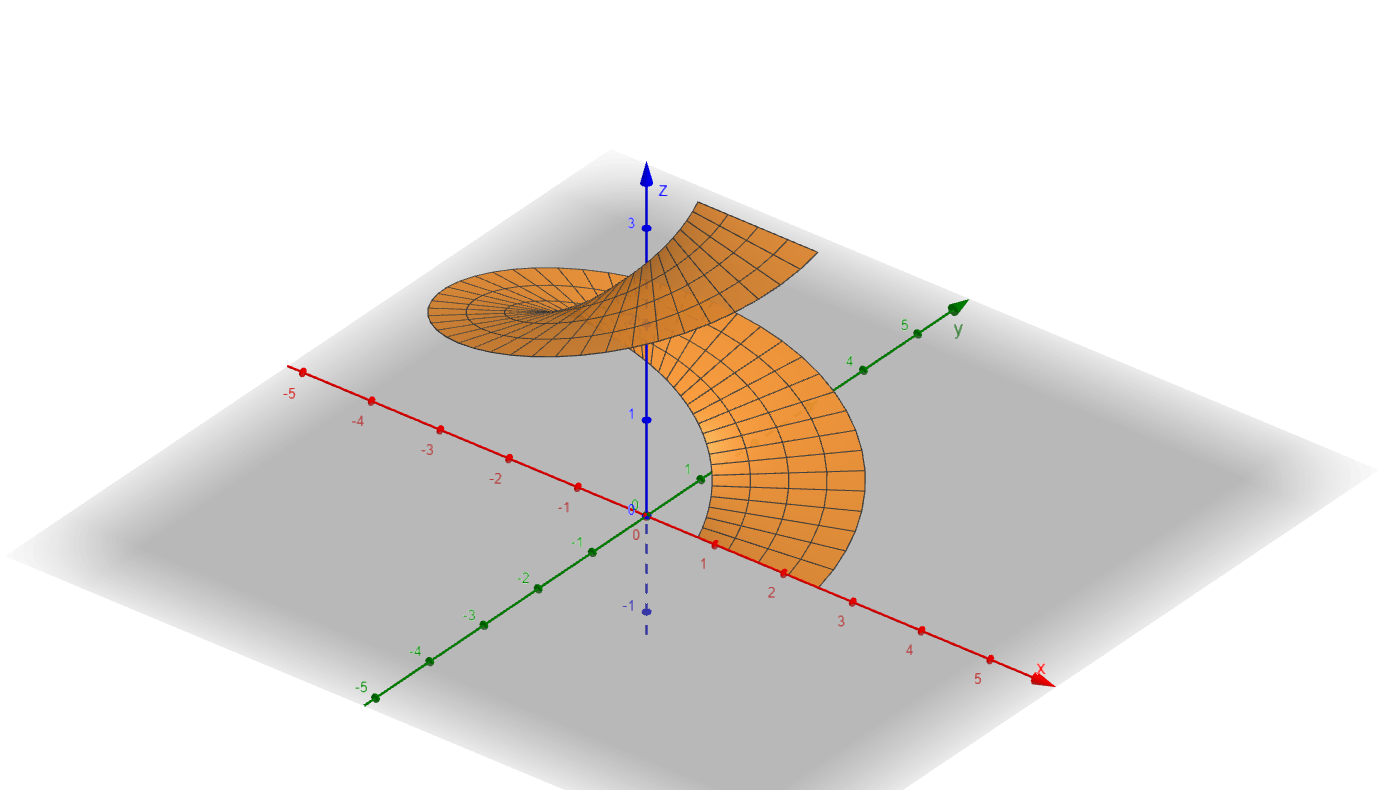
\includegraphics[width=0.7\linewidth]{figures_tech/ct.png} 
	\caption{Bài toán 3}
	\label{fig:stairs_real}
\end{figure}

\subsubsection{Lời giải chi tiết bằng giải tích}

Đầu tiên, ta sẽ dựng công thức bề dày bê tông chạy theo tham số u vì đây là tham số chạy theo bề rộng thang. Đặt biến H là độ dày bê tông tại 1 điểm trên thang:
\begin{equation}
	H(u)=au+b
\end{equation}
Theo đề bài ta có: $H(1)=0.35$; $H(2.5)=0.25$
\[
\Rightarrow a=-\frac{1}{15}; \qquad b=\frac{5}{12}
\]
Thay vào, ta có hàm bề dày:
\begin{equation}
	H(u)=-\frac{1}{15}u+\frac{5}{12}
\end{equation}
Tiếp theo, ta lập hàm tính thể tích bê tông bằng cách lấy bề dày tại từng điểm trên mặt nhân với vi phân diện tích mặt tại điểm đó và tích phân trên cả mặt cong:
\begin{equation}
	V=\iint_{S} H \cdot dS
\end{equation}
với vi phân diện tích dS ta đổi thành tính trên vi phân diện tích hình học phẳng miền D, ta chuyển tích thành:
\begin{equation}
	V=\int_{0}^{2\pi}\int_{1}^{2.5}H(u) \cdot |\vec{r}_{u}\times\vec{r}_{v}| \cdot dudv
\end{equation}
mà:
\begin{align}
	\vec{r}_{u} &= (\cos(v), \sin(v), 0) \\
	\vec{r}_{v} &= \left(-u\sin(v), u\cos(v), \frac{3.5}{2\pi}\right)
\end{align}
\begin{equation}
	\Rightarrow \vec{r}_{u}\times\vec{r}_{v} = \left(\frac{3.5}{2\pi}\sin(v), -\frac{3.5}{2\pi}\cos(v), u\cos^2(v)+u\sin^2(v)\right) = \left(\frac{3.5}{2\pi}\sin(v), -\frac{3.5}{2\pi}\cos(v), u\right)
\end{equation}
\begin{equation}
	\Rightarrow |\vec{r}_{u}\times\vec{r}_{v}| = \sqrt{\left(\frac{3.5}{2\pi}\sin(v)\right)^2 + \left(-\frac{3.5}{2\pi}\cos(v)\right)^2 + u^2} = \sqrt{u^2 + \left(\frac{3.5}{2\pi}\right)^2}
\end{equation}
Thay vào tích phân:
\begin{equation}
	V = \int_{0}^{2\pi}\int_{1}^{2.5} \left(-\frac{1}{15}u+\frac{5}{12}\right) \cdot \sqrt{u^2 + \left(\frac{3.5}{2\pi}\right)^2} \cdot dudv
\end{equation}
vì hàm tích phân theo u độc lập hoàn toàn với biến v nên tách tích phân lớp ngoài ra trước:
\begin{equation}
	V = \int_{0}^{2\pi}dv \cdot \int_{1}^{2.5} \left(-\frac{1}{15}u+\frac{5}{12}\right) \cdot \sqrt{u^2 + \left(\frac{3.5}{2\pi}\right)^2} \cdot du = 2\pi \cdot \int_{1}^{2.5} \left(-\frac{1}{15}u+\frac{5}{12}\right) \cdot \sqrt{u^2 + \left(\frac{3.5}{2\pi}\right)^2} \cdot du
\end{equation}
Bấm máy tính (hoặc tính toán giải tích) phần tích phân biến u ta được:
\begin{equation}
	V \approx 2\pi \cdot 0.81099 \approx 5.0956 \; (m^3)
\end{equation}
Có thể tích, khối lượng cầu thang là:
\begin{equation}
	M = D \cdot V \approx 2500 \cdot 5.0956 \approx 12739 \; (kg)
\end{equation}
Vậy khối lượng bê tông cốt thép xấp xỉ gần 13 tấn.

\subsubsection{Kết quả mô phỏng matlab}
Đoạn mã MATLAB thực hiện quá trình khai báo hàm vector tham số bề mặt kết hợp ứng dụng tích phân số trị bậc cao đã cho ra kết quả dung tích khối khớp hoàn toàn với giá trị tính toán lý thuyết giải tích là $V \approx 5.0956~m^3$, qua đó quy đổi chính xác tải trọng vật liệu đạt ngưỡng gần $13$ tấn.

\begin{figure}[H]
	\centering
 	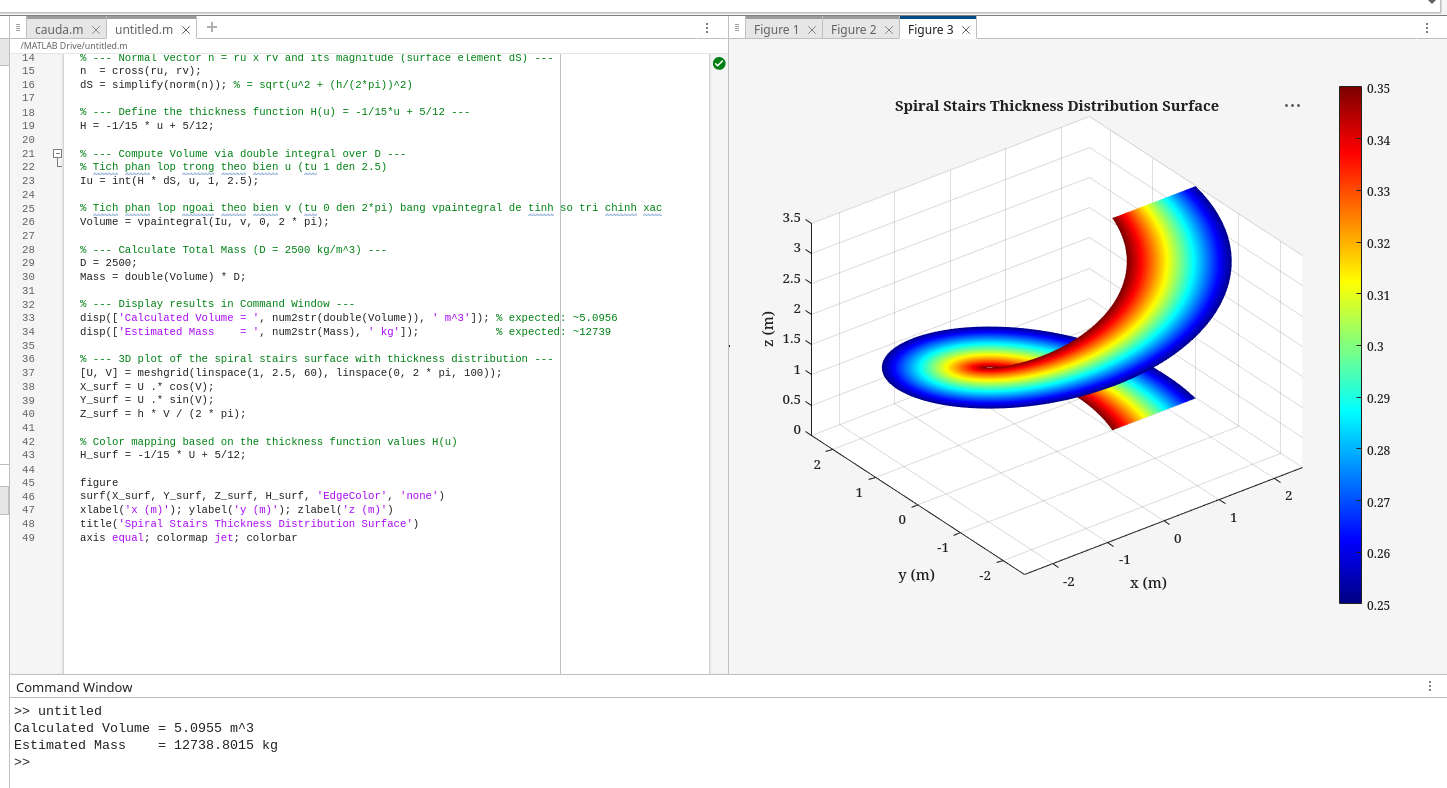
\includegraphics[width=1.0\linewidth]{figures_tech/bt3.png} 
	\caption{Mô phỏng Matlab bài toán 3}
	\label{fig:matlab_stairs}
\end{figure}

% =========================================================
\newpage
\renewcommand{\refname}{Tài liệu tham khảo}
\begin{thebibliography}{10}
	
	% --- Giáo trình và tài liệu tiếng Việt ---
	\bibitem{gt2_hcmut} 
	Bộ môn Toán Ứng dụng -- Trường Đại học Bách Khoa, ĐHQG-HCM, 
	\textit{Giáo trình Giải tích 2}. 
	TP.HCM: Nhà xuất bản Đại học Quốc gia TP.HCM.
	
	
	\bibitem{baitap_toancaocap_tap3} 
	N.~Đ.~Trí (Chủ biên), 
	\textit{Bài tập Toán học cao cấp -- Tập 3: Phép tính Giải tích nhiều biến số}. 
	Hà Nội: Nhà xuất bản Giáo dục Việt Nam, 2015.
	
	% --- Giáo trình tiếng Anh chuẩn quốc tế ---
	\bibitem{stewart_calculus} 
	J.~Stewart, 
	\textit{Calculus: Early Transcendentals}, 8th~ed. 
	Boston, MA: Cengage Learning, 2015.
	
	\bibitem{thomas_calculus} 
	G.~B.~Thomas, M.~D.~Weir, và J.~Hass, 
	\textit{Thomas' Calculus}, 13th~ed. 
	Boston, MA: Pearson, 2014.
	
	\bibitem{kreyszig_math}
	E.~Kreyszig, 
	\textit{Advanced Engineering Mathematics}, 10th~ed. 
	Hoboken, NJ: John Wiley \& Sons, Inc., 2011.
	
	\bibitem{larson_calculus}
	R.~Larson và B.~H.~Edwards, 
	\textit{Calculus}, 11th~ed. 
	Boston, MA: Cengage Learning, 2018.
	
	% --- Tài liệu kỹ thuật phần mềm (MATLAB) ---
	\bibitem{matlab_symbolic} 
	MathWorks, 
	``Symbolic Math Toolbox User's Guide,'' 
	\textit{MathWorks, Inc.} [Trực tuyến]. 
	Địa chỉ: \url{https://www.mathworks.com/help/symbolic/}
	
	\bibitem{matlab_surface} 
	MathWorks, 
	``3-D Surface Plots,'' 
	\textit{MathWorks, Inc.} [Trực tuyến]. 
	Địa chỉ: \url{https://www.mathworks.com/help/matlab/visualize/representing-a-matrix-as-a-surface.html}
	
	\bibitem{matlab_integral} 
	MathWorks, 
	``Integration and Calculus in MATLAB,'' 
	\textit{MathWorks, Inc.} [Trực tuyến]. 
	Địa chỉ: \url{https://www.mathworks.com/help/matlab/math/integration-and-calculus.html}
	
\end{thebibliography}

% =========================================================
\newpage
\appendix
\section{Phụ lục - Mã nguồn MATLAB}
\subsection{Mã nguồn cho Bài toán 1: Đường hầm núi tuyết}
\begin{lstlisting}[language=Matlab, frame=single, numbers=left, numberstyle=\tiny\color{gray}, basicstyle=\ttfamily\small, breaklines=true, backgroundcolor=\color{gray!5}, keywordstyle=\color{blue}, commentstyle=\color{green!60!black}, stringstyle=\color{purple}]
	syms x y
	
	% --- Define the surface z = sqrt(1 - x^2) ---
	z = sqrt(1 - x^2);
	
	% --- Compute partial derivatives ---
	dz_dx = diff(z, x);
	dz_dy = diff(z, y);     % equals 0 (z does not depend on y)
	
	% --- Surface element dS = sqrt(1 + dz_dx^2 + dz_dy^2) ---
	dS = simplify(sqrt(1 + dz_dx^2 + dz_dy^2));
	
	% --- Upper bound for y: from y = 0 to y = 2 - z ---
	y_upper = 2 - z;
	
	% --- Define the cost function C(x, y, z) = 100 + 50y ---
	C = 100 + 50 * y;
	
	% --- Compute total cost via iterated integral ---
	%   inner integral: y from 0 to y_upper
	%   outer integral: x from -1 to 1
	Total_Cost = int(int(C * dS, y, 0, y_upper), x, -1, 1);
	Total_Cost = simplify(Total_Cost);
	
	% --- Display results in Command Window ---
	disp(['Symbolic Total Cost = ', char(Total_Cost)]);  % expected: (625*pi)/2 - 400
	disp(['Numeric Total Cost  = ', num2str(double(Total_Cost)), ' million VND']);
	
	% --- 3D plot of the tunnel surface with cost distribution ---
	[U, V] = meshgrid(linspace(-1, 1, 80), linspace(0, 2, 60));
	Z_surf = sqrt(1 - U.^2);
	Y_surf = V;
	mask   = (Y_surf >= 0) & (Y_surf <= 2 - Z_surf);
	Z_surf(~mask) = NaN;
	
	% Color mapping based on the cost function values
	C_surf = 100 + 50 * Y_surf; 
	
	figure
	surf(U, Y_surf, Z_surf, C_surf, 'EdgeColor', 'none')
	xlabel('x (m)'); ylabel('y (m)'); zlabel('z (m)')
	title('Snow-mountain Tunnel Cost Distribution Surface')
	axis equal; colormap jet; colorbar
\end{lstlisting}
\newpage
\subsection{Mã nguồn cho Bài toán 2: Mô hình cầu đá}
\begin{lstlisting}[language=Matlab, frame=single, numbers=left, numberstyle=\tiny\color{gray}, basicstyle=\ttfamily\small, breaklines=true, backgroundcolor=\color{gray!5}, keywordstyle=\color{blue}, commentstyle=\color{green!60!black}, stringstyle=\color{purple}]
	syms u v
	% --- Parametric surface: half-cylinder x^2 + z^2 = 1, z >= 0 ---
	%   x = cos(u),  z = sin(u),  y = v
	%   u in [0, pi]   (upper half: z >= 0)
	%   v in [1, 2]    (between the two planes y = 1 and y = 2)
	r = [cos(u), v, sin(u)];    % position vector [x, y, z]
	
	% --- Tangent vectors ---
	ru = diff(r, u);    % dr/du = [-sin(u), 0,  cos(u)]
	rv = diff(r, v);    % dr/dv = [      0, 1,       0]
	
	% --- Normal vector n = ru x rv and its magnitude (surface element dS) ---
	n  = cross(ru, rv);         % = [-cos(u), 0, -sin(u)]
	dS = simplify(norm(n));     % = 1  (from the Pythagorean identity)
	
	% --- Define the cost function C(x, y, z) = 61 + 73y + 12z ---
	% Thay the x = cos(u), y = v, z = sin(u) vao ham chi phi
	C = 61 + 73 * v + 12 * sin(u);
	
	% --- Total cost via double integral over D ---
	%   inner integral: u from 0 to pi
	%   outer integral: v from 1 to 2
	Total_Cost = int(int(C * dS, u, 0, pi), v, 1, 2);
	Total_Cost = simplify(Total_Cost);
	
	% --- Display results in Command Window ---
	disp(['Symbolic Total Cost = ', char(Total_Cost)]);  % expected: 170.5*pi + 24
	disp(['Numeric Total Cost  = ', num2str(double(Total_Cost)), ' million VND']);
	
	% --- 3D plot of the stone-arch bridge surface with cost distribution ---
	[U, V]  = meshgrid(linspace(0, pi, 80), linspace(1, 2, 40));
	X_surf  = cos(U);
	Y_surf  = V;
	Z_surf  = sin(U);
	
	% Color mapping based on the cost function values
	C_surf  = 61 + 73 * Y_surf + 12 * sin(U);
	
	figure
	surf(X_surf, Y_surf, Z_surf, C_surf, 'EdgeColor', 'none')
	xlabel('x (m)'); ylabel('y (m)'); zlabel('z (m)')
	title('Stone-arch Bridge Cost Distribution Surface')
	axis equal; colormap jet; colorbar
\end{lstlisting}

\newpage 

% ---------------------------------------------------------
\subsection{Mã nguồn cho Bài toán 3: Bài toán Cầu thang}
\begin{lstlisting}[language=Matlab, frame=single, numbers=left, numberstyle=\tiny\color{gray}, basicstyle=\ttfamily\small, breaklines=true, backgroundcolor=\color{gray!5}, keywordstyle=\color{blue}, commentstyle=\color{green!60!black}, stringstyle=\color{purple}]
	syms u v
	
	% --- Parametric surface: Helicoide (Stone stairs) ---
	%   x = u*cos(v),  y = u*sin(v),  z = h*v/(2*pi)
	%   u in [1, 2.5]   (be rong bac thang)
	%   v in [0, 2*pi]  (vong xoan cua thang)
	h = 3.5;
	r = [u * cos(v), u * sin(v), h * v / (2 * pi)];
	
	% --- Tangent vectors ---
	ru = diff(r, u);    % dr/du = [cos(v), sin(v), 0]
	rv = diff(r, v);    % dr/dv = [-u*sin(v), u*cos(v), h/(2*pi)]
	
	% --- Normal vector n = ru x rv and its magnitude (surface element dS) ---
	n  = cross(ru, rv);
	dS = simplify(norm(n)); % = sqrt(u^2 + (h/(2*pi))^2)
	
	% --- Define the thickness function H(u) = -1/15*u + 5/12 ---
	H = -1/15 * u + 5/12;
	
	% --- Compute Volume via double integral over D ---
	% Tich phan lop trong theo bien u (tu 1 den 2.5)
	Iu = int(H * dS, u, 1, 2.5);
	
	% Tich phan lop ngoai theo bien v (tu 0 den 2*pi) bang vpaintegral de tinh so tri chinh xac
	Volume = vpaintegral(Iu, v, 0, 2 * pi);
	
	% --- Calculate Total Mass (D = 2500 kg/m^3) ---
	D = 2500;
	Mass = double(Volume) * D;
	
	% --- Display results in Command Window ---
	disp(['Calculated Volume = ', num2str(double(Volume)), ' m^3']); % expected: ~5.0956
	disp(['Estimated Mass    = ', num2str(Mass), ' kg']);            % expected: ~12739
	
	% --- 3D plot of the spiral stairs surface with thickness distribution ---
	[U, V] = meshgrid(linspace(1, 2.5, 60), linspace(0, 2 * pi, 100));
	X_surf = U .* cos(V);
	Y_surf = U .* sin(V);
	Z_surf = h * V / (2 * pi);
	
	% Color mapping based on the thickness function values H(u)
	H_surf = -1/15 * U + 5/12;
	
	figure
	surf(X_surf, Y_surf, Z_surf, H_surf, 'EdgeColor', 'none')
	xlabel('x (m)'); ylabel('y (m)'); zlabel('z (m)')
	title('Spiral Stairs Thickness Distribution Surface')
	axis equal; colormap jet; colorbar
\end{lstlisting}

